%%%% Metología propuesta

\chapter{Metodología}
\section{Plan de Actividades}

Con el fin de cumplir con lo planteado para el proyecto se diseña el cronograma mostrado en la en la figura \ref{fig:crono}.

%\begin{center} ARREGLAR POR NUEVAS COSAS 
\begin{figure}[ht!]
\begin{centering}
%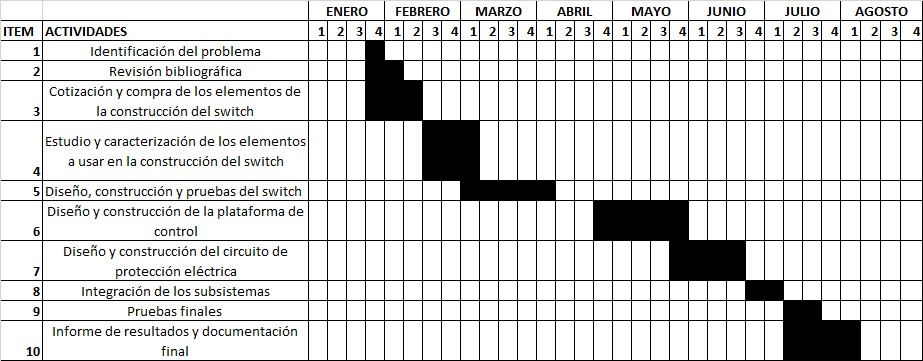
\includegraphics [angle=90]{Images/Cronograma}
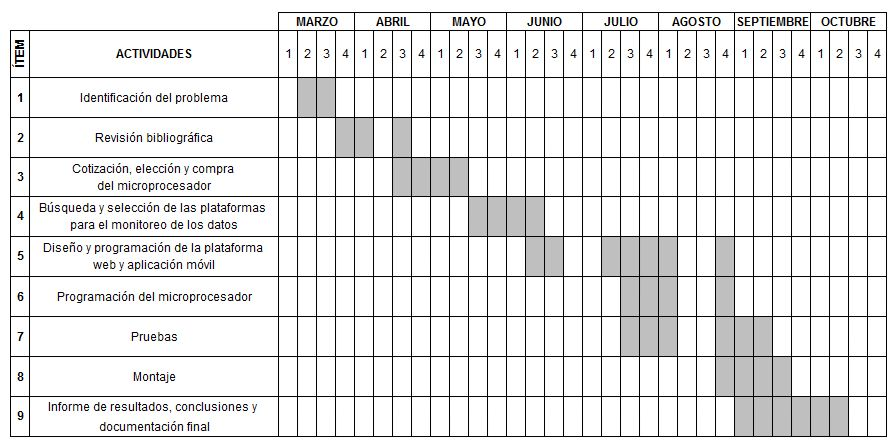
\includegraphics [trim = 0mm 0mm 0mm 0mm, clip,angle=0,scale=0.65]{Images/crono}%trim recorta izquierda abajo derecha arriba
%\par\end{centering}
\caption{\label{fig:crono}Cronograma de actividades}
\textit{Fuente: Autores}. 
\par\end{centering}
\end{figure}
%\par
%\end{center}

%\begin{figure}[ht]
%\caption{\label{fig:Cronograma} Cronograma de actividades}
%\begin{centering}
%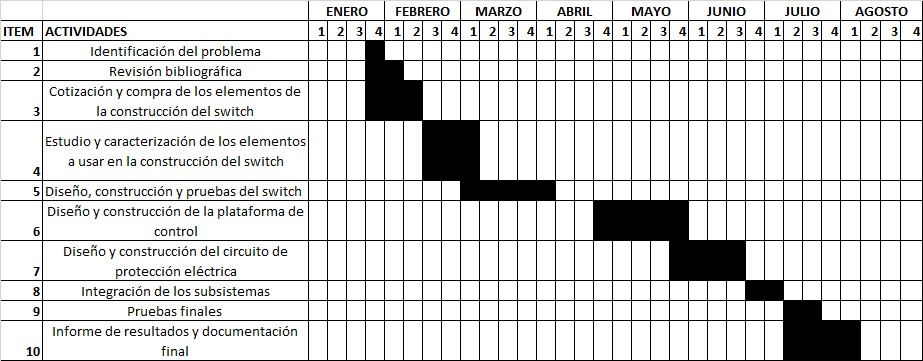
\includegraphics [trim = 0mm 3mm 0mm 0mm, clip,angle=0,scale=0.75]{Images/Cronograma}
%\textit{Fuente: Autor}.
%\par \end{centering}
%\end{figure}


\subsection{Identificación del problema}

Se revisa el problema planteado, el cual es el uso de manera remota del prototipo previamente diseñado\cite{Paneles}\cite{Proto}, para así facilitar el acceso a los datos en tiempo real de sus diferentes sensores y el control a distancia del mismo.

\subsection{Revisión bibliográfica}

Se inventiga de libros, artículos acerca de IoT (Internet of Things), proyectos de grado y material de consulta en general, para conseguir una amplia cantidad de información, y así tener la documentación necesaria para iniciar el proyecto.

\subsection{Cotización, elección y compra de microprocesador}

En esta etapa, se investiga acerca de los diferentes tipos de microprocesadores que cumplan con las especificaciones requeridas, luego de esto, se realiza las respectivas cotizaciones y se elige el más adecuado para trabajar en este proyecto.

\subsection{Búsqueda y selección de plataformas para el monitoreo de los datos}

La idea principal de este proyecto, es poder visualizar las variables medidas a través de una plataforma \textit{WEB} y/o una aplicación móvil, para esto, se investiga acerca de los diferentes métodos para diseñar estas herramientas y se selecciona la más adecuada.

\subsection{Diseño y programación de la plataforma \textit{WEB} y aplicación móvil}

Se diseñan las plataformas para la visualización de las variables, tanto la página \textit{WEB}, como la aplicación para móviles, con ayuda de herramientas disponibles en la WEB, usadas en IoT.

\subsection{Progamación del microprocesador}

Se programa el microprocesador elegido, para que realice la recepción de los datos desde el prototipo anteriormente mencionado y los transmita de manera inalámbrica por WIFI.  

\subsection{Pruebas}

Con el fin de realizar ajustes necesarios y detectar posibles errores, se realizan las pruebas suficientes para determinar la eficiencia del sistema.

\subsection{Montaje}

Se lleva a cabo el montaje de todos los elementos a usar y se arreglan los últimos detalles para la entrega final del componente. 

\subsection{Informe de resultados, conclusiones y documentación final }

En esta etapa final, se recopilan los resultados, los problemas encontrados, el análisis realizado y solución, además de las conclusiones obtenidas durante el desarrollo del proyecto y se consignan en el documento final; esto se realiza simultáneamente con las etapas mencionadas anteriormente.

\section{Diagrama de bloques}

Para la realización de este proyecto, se plantea el diagrama de bloques de la figura \ref{fig:bloques}, donde se puede visualizar las conexiones entre el prototipo y el microprocesador con módulo WIFI, y a su vez los elementos en donde se podrá acceder a los datos transmitidos.

\begin{figure}[ht!]
\begin{centering}
%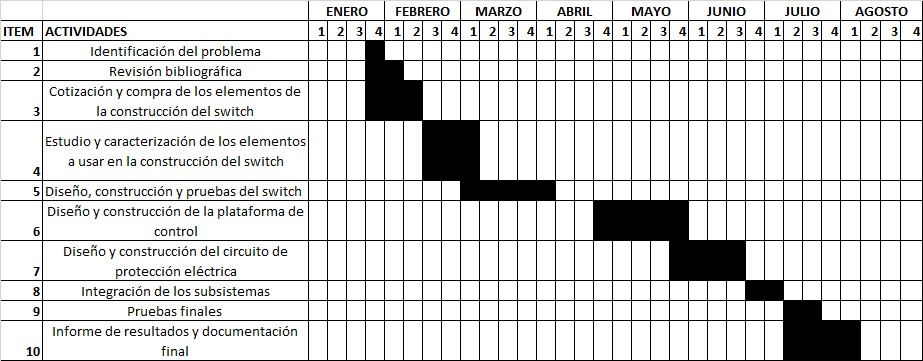
\includegraphics [angle=90]{Images/Cronograma}
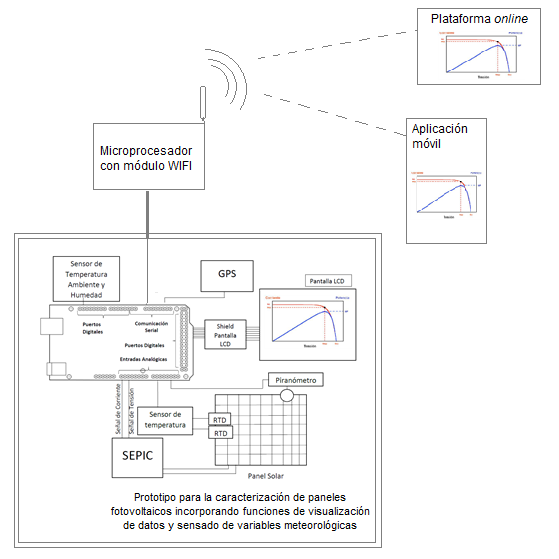
\includegraphics [trim = 0mm 0mm 0mm 0mm, clip,angle=0,scale=0.65]{Images/bloques}%trim recorta izquierda abajo derecha arriba
%\par\end{centering}
\caption{\label{fig:bloques}Diagrama de bloques de la solución.}
\textit{Tomada de \cite{Proto}, editada por autores.} 
\par\end{centering}
\end{figure}

\section{Resultados Esperados}

Al finalizar el proyecto se espera obtener una plataforma \textit{online} y una aplicación móvil, ambas para el monitoreo de los datos obtenidos por medio del prototipo; para esto se debe asegurar el apropiado funcionamiento de los elementos instalados. Con base a esto los entregables e informes basados en los objetivos específicos se plantean se la siguiente manera: 

\begin{itemize}
\item Entregar plataforma de monitoreo \textit{online} y aplicación móvil funcionado correctamente.

\item Almacenamiento de los datos medidos por el prototipo, ya sea en una base de datos en la nube o en una unidad de almacenamiento en un computador y además una correcta trasmisión de los datos.

\item Realizar montaje del sistema de desarrollo con WIFI y su comunicación con el prototipo.

\end{itemize}

\section{Recursos e infraestructura}

Para llevar a cabo el proyecto se plantean los recursos humanos e infraestructura mostrados en la tabla \ref{tab:Recurso-humano} y la tabla \ref{tab:Resumen-costos-equipo} respectivamente. 

%\begin{table}[ht!]
\begin{table}[ht]
\caption{\label{tab:Recurso-humano} Recurso humano}
\begin{centering}
\begin{tabular}{|c||c||c|}
\hline 
Función  & Horas/Sem & Dedicación Total
\tabularnewline
\hline
\hline 
Director del Proyecto & 1 & 24 \tabularnewline % areglar horas 
\hline 
\hline
Codirector del Proyecto & 1 & 24 \tabularnewline %% areglar horas 
\hline 
\hline
Autores & 16  & 384 \tabularnewline %%areglar horas
\hline
\hline
\end{tabular}
\par \end{centering}
\end{table}
%\end{center}

%\begin{center}
\begin{table}[ht]
\caption{\label{tab:Resumen-costos-equipo} Equipo, software e insumos}
\begin{centering}
\begin{tabular}{|c||c||c|}
\hline 
\textbf{Descripción} & \textbf{Cantidad} & \textbf{Justificación} \tabularnewline
\hline
\hline 
 &  &  Almacenamiento de Información\tabularnewline
Equipos  & 2 & Programación del microprocesador \tabularnewline
 de Cómputo &  & Interfaz de monitoreo \tabularnewline & & Diseño y visualización   \tabularnewline
 \hline
 \hline
Microprocesador  & 1 & Recepción y transmisión de datos   \tabularnewline
\hline  
\hline
Celular  & 1 &  Visualización de aplicacion de monitoreo\tabularnewline
\hline 
\hline
Papelería & Global & Presentación de informes y papeleo necesario  \tabularnewline 
\hline 
\hline
Prototipo de caracterización &  &  \tabularnewline 
de paneles fotovoltaicos y medición & 1 & Medición de variables \tabularnewline 
de variables metereológicas & & \tabularnewline 
\hline
\hline
Memoria externa  & 1 & Almacenamiento de información\tabularnewline
\hline
\hline
Acceso a bases de datos & Global & Busqueda de información \tabularnewline
\hline
\hline
\end{tabular}
\par\end{centering}
\end{table}


\newpage
\chapter{Reseña bibliográfica}

Cuando hablamos de IoT, pensamos en los teléfonos móviles como centro de diferentes operaciones, por ello Paul Jacobs, ex jefe ejecutivo de Qualcomm, ha dicho:''En el futuro, casi todas las cosas estarán enlazadas en la web, y los teléfonos móviles funcionarán como centros de actividades para IoT. Por lo tanto, IoT es nada más que la conexión a Internet de objetos inteligentes y sistemas embebidos, con teléfonos móviles como centros de acceso''. Los objetos inteligentes se pueden describir como cosas u objetos que son responsables de proporcionar información útil sobre sus interacciones en una red. Estos objetos se pueden desplegar en una red vía Bluetooth Baja Energía (IEEE 802.15.4), Wi-Fi (IEEE 802.11), Ethernet (IEEE 802.3) u otro tipo de protocolo de comunicación.

Las posibilidades de desarrollo que ofrece IoT tanto en hardware como en software son infinitas. El hardware IoT puede clasificarse en dos categorías amplias: dispositivos y aparatos portátiles y
sistemas embebidos y tarjetas, como se muestra en la Figura 4.1.
En la categoría de portátiles, se encuentran muchos aparatos hoy en día, que van desde zapatos inteligentes, gafas y hasta relojes que sirven para recibir llamadas.
Por otro lado, tanto los aspectos de hardware como de software están abiertos para los desarrolladores bajo los sistemas embebidos y
tarjetas de desarrollo. Los servicios prestados por estos sistemas y
tarjetas pueden ser clasificados en tres subcategorías: control de dispositivos, adquisición de datos, y aplicaciones de desarrollo. El control de dispositivos incluye la supervisión de dispositivos, seguridad y actualizaciones de software. La adquisición de datos abarca la gestión y transformación de información en diferentes capas del IoT. Por último, el desarrollo de aplicaciones incluye análisis, lógica impulsada por eventos, visualización y programación de aplicaciones.\cite{7879392}

\begin{figure}[ht!]
\begin{centering}
%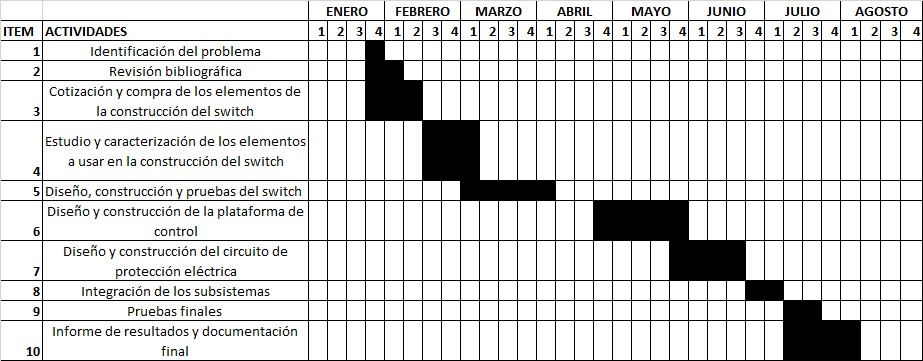
\includegraphics [angle=90]{Images/Cronograma}
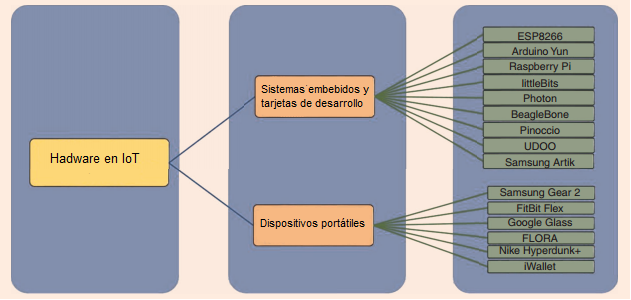
\includegraphics [trim = 0mm 0mm 0mm 0mm, clip,angle=0,scale=0.6]{Images/hadware}%trim recorta izquierda abajo derecha arriba
\caption{\label{fig:Hadware}Clasificación del Hadware en IoT} \textit{Tomada de: ''Create Your Own Internet of Things'', por K.J.Singh and D.S.Kapoor, 2017, IEEE Consumer Electronics Magazine , Vol 6 No.2, p. 57-68.}
\par\end{centering}
\end{figure}

En cuanto al software en IoT, se cuenta con una amplia gama de herramientas, con diferentes tipos de lenguaje, como C, C++, python,entre otros. Existen muchas plataformas de software IoT dsiponibles en el mercado para simplificar y acelerar el proceso de enviar y/o recibir información, proporcionan marcos de programación máquina a máquina (M2M), gestión de datos y de dispositivos, seguridad, almacenamiento y traducción de protocolos. Muchas de estas herramientas cuentan con diferentes servicios como por ejemplo, que cuando se produzca un evento específico en el mundo real, se emita una notificación mediante correo electrónico o mensaje de texto. 

La selección de una plataforma de software IoT es una parte crítica del desarrollo de productos IoT. Es esencial saber qué plataforma de software IoT soportará una plataforma de hardware IoT específica. La elección de una plataforma de software óptima será impulsada por los instrumentos proporcionados, específicamente, el IDE para la programación y la API disponible para el acceso de datos y notificaciones.
Además, la eficiencia de las herramientas de gestión de datos, tales como aplicaciones de escritorio y móviles, cuadros de mando y similares, también hace que la elección particular sea significativa. Por último, los precios, el apoyo de la comunidad y la documentación disponible también deben tenerse en cuenta al seleccionar una plataforma de software.\cite{7879392}

\nocite{7925808}
\nocite{7842386}
\nocite{esp32}
\nocite{omega}
\nocite{raspberry}
\nocite{molano}
\nocite{Cha}
\nocite{thingspeak}
\nocite{initial}
\nocite{ubidots}


\begin{figure}[ht!]
\begin{centering}
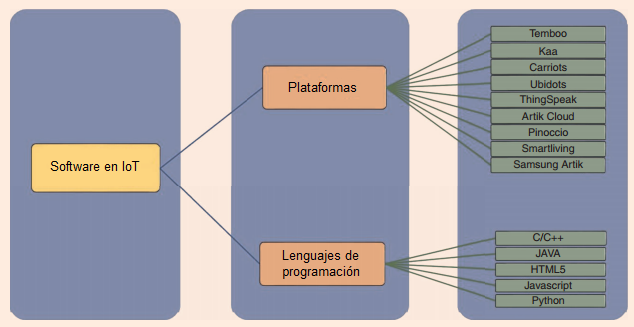
\includegraphics [trim = 0mm 0mm 0mm 0mm, clip,angle=0,scale=0.55]{Images/software}%trim recorta izquierda abajo derecha arriba
\caption{\label{fig:Software}Clasificación del software en IoT} \textit{Tomada de: ''Create Your Own Internet of Things'', por K.J.Singh and D.S.Kapoor, 2017, IEEE Consumer Electronics Magazine , Vol 6 No.2, p. 57-68.}
\par\end{centering}
\end{figure}
